% 181-14(181쪽) — 한 변의 길이가 6인 정삼각형과 각 변의 중점을 이어 그린 정삼각형(1회 시행).
% 스캔 그림이라 화질이 낮아 TikZ 로 다시 그렸다. 원문에 있는 6 만 적고 8회 시행의 둘레(답)는 적지 않는다.
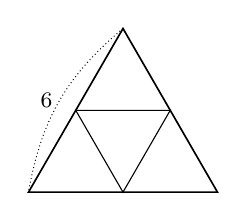
\begin{tikzpicture}[scale=0.4, line width=0.6pt]
  \coordinate (B) at (0,0);
  \coordinate (C) at (6,0);
  \coordinate (A) at (3,5.196);
  \coordinate (M) at (1.5,2.598);
  \coordinate (N) at (4.5,2.598);
  \coordinate (L) at (3,0);
  \draw (A) -- (B) -- (C) -- cycle;
  \draw[line width=0.4pt] (M) -- (N) -- (L) -- cycle;
  \draw[densely dotted, line width=0.35pt] (A)
    to[bend right=20] node[midway, left=-1pt, font=\footnotesize] {$6$} (B);
\end{tikzpicture}
